\documentclass{article}
\usepackage{graphicx}
\usepackage{caption}
\usepackage{float}
\usepackage[arrowdel]{physics}
\usepackage{amsmath}
\usepackage{amsfonts}
\usepackage{amsthm}
\DeclareMathOperator*{\argmax}{arg\,max}
\def\ind{\hspace{\parindent}}
\title{Brief Report}
\author{Amirreza Negari, Amirhossein Estiri, Sajad Kahani}
\date{Augest 2019}
\begin{document}

\maketitle

\section{Optimization Problem}
let ${\lambda_1..\lambda_m}$ be set of free degrees of Hamiltonian, $\ket{\phi_0}$ the ground state and $\ket{\psi}$ the target state.

formally, problem can be formulated by this equation
\[ H^*, t^* = \argmax_{\lambda_1..\lambda_m, t} \mathcal{F}(e^{iHt} \ket{\phi_0}, \ket{\psi}) \]

where $\mathcal{F}(., .)$ is fidelity.

specifically, we are focusing on a Hisenberg model, therefore

\[ H = \sum_{i=1}^{N-1} J_i X_i X_{i+1} + \sum_{i=1}^N B_i Z_i\]

\begin{equation} 
\label{eq:opt}
H^*, t^* = \argmax_{J_1..J_{N-1}, B_1..B_N, t} \mathcal{F}(e^{iHt} \ket{\phi_0}, \ket{\psi})
\end{equation}

\section{Numerical Optimization}
\subsection{One-sector Subspace}
For the one-sector subspace, we can write $H$ as a parameteric matrix. then eq. \ref{eq:opt} can be solved approximately using gradient-descent method by a deep-learning framework.

This approach is the same as what Innocenti. et. al. did for gate construction.


\newtheorem{lemma}{Lemma}
\begin{lemma}
we define a mapping $\mathbb{R}^{2N} \rightarrow \mathbb{C}^{N}$ as $f(v) = \sum_{i=1}^N (v_{2i} + iv_{2i+1}) \ket{i}$ \\
if $\va{v}\cdot\va{v'} = 1 - \epsilon$, where $\epsilon \ll 1$, then $\braket{f(v)}{f(v')} = 1 - 2\epsilon + O(\epsilon^2)$

proof:

\[ \va{v}\cdot\va{v'} = 1 - \epsilon \Rightarrow |\va{v} - \va{v'}|\]

\begin{align*} \braket{f(v)}{f(v')} &= \sum_{i=1}^N f(v')_i^* f(v)_i = \sum_{i=1}^N (v_{2i} - iv_{2i+1}) (v'_{2i} + iv'_{2i+1}) \\
& = \sum_{i=1}^N v_{2i}v'_{2i} + v_{2i+1}v'_{2i+1} +  \sum_{i=1}^N i(v_{2i}v'_{2i+1} - v'_{2i}v_{2i+1}) \\
& = \va{v}\cdot\va{v'} + \sum_{i=1}^N i(v_{2i}v'_{2i+1} - v_{2i}v_{2i+1} + v_{2i}v_{2i+1}- v'_{2i}v_{2i+1}) \end{align*}

\[ v_r.dv_i + v_r.v_i - v_i.v'_r \]

\end{lemma}

\begin{lemma}
if
$H = U^\dagger D U$
\[ \pdv{H^k}{H_{mn}} = \sum_{1 \le i, j, \alpha,\beta \le \dim{\mathcal{H}}} U_{m\alpha}^\dagger U_{j\beta}^\dagger U_{\alpha i} U_{\beta n} \frac{D_{\alpha\alpha}^k - D_{\beta\beta}^k}{D_{\alpha\alpha} - D_{\beta\beta}} \dyad{i}{j} \] 
\end{lemma}

here are results of applying this method on a one-sector space with aforementioned Hamiltonain, where $\ket{\phi_0} = \ket{1}$ and $\ket{\psi}$ are just random vectors.

\begin{figure}[H]
\centering
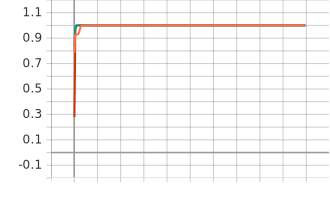
\includegraphics[width=0.4\textwidth]{fidelity_4}
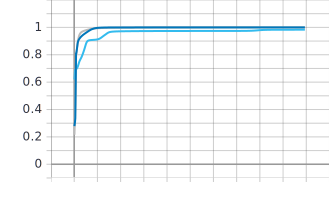
\includegraphics[width=0.4\textwidth]{fidelity_8} \\
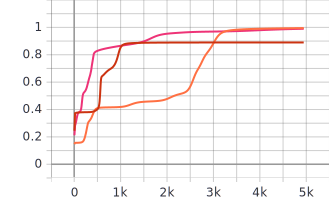
\includegraphics[width=0.4\textwidth]{fidelity_16}
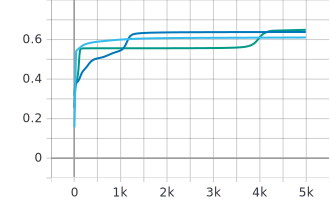
\includegraphics[width=0.4\textwidth]{fidelity_32}
\caption{fidelity vs. number of cycles for different random target vectors. 
\\ a) $\dim \mathcal{H} = 4$, b) $\dim \mathcal{H} = 8$, c) $\dim \mathcal{H} = 16$, d) $\dim \mathcal{H} = 32$
\\ Note. all of plots have the same x axis.}
\end{figure}

\end{document}